\section{Experiment 4. 03.03.2020}\label{experiment-4.-03.03.2020}

It took place on 03.03.2020. The weather conditions were appropriate for the experiment, although there was raining lightly.

For the fourth trial, we implement sending of measurement messages only with \gls{http} protcol from \gls{ue} to \gls{command_n_center}. 

We aimed to find optimized positions for the \glspl{ue} in three cases (Sub-Optimal, Uniform, Near-Optimal).

We decided to reduce the area layout to 25x25 meters.

We use one smartphone with a special program that can precisely locate the position. Then we placed the phone where \glspl{ue} and \glspl{ap} were, which helped us to find out the initial positions. These coordinates for \glspl{ue} are shown in Table \ref{tab:exp4-initial-coordinates-ues}. We use \texttt{decimal degrees} for coordinates.

\begin{longtable}[]{@{}ll@{}}
	\caption{Initial coordinates for \glspl{ue}}\tabularnewline
	\toprule
	Unique ID & Coordinates\tabularnewline
	\midrule
	\endhead
	f072f812f48ce468 & 50.6823458, 10.94051806\tabularnewline
	eb0b54819c69cf0c & 50.6824625, 10.9403367\tabularnewline
	27349a2cde6592df & 50.6822786, 10.94057\tabularnewline
	51336504999bc1ca & 50.6822861, 10.940590\tabularnewline
	b1c225280d0ed13f & 50.6824403, 10.940343889\tabularnewline
	abb76773bdee4fa0 & 50.6824789, 10.940261944\tabularnewline
	\label{tab:exp4-initial-coordinates-ues}
\end{longtable}


The initial coordinates for \glspl{ap} are shown in Table \ref{tab:exp4-initial-coordinates-aps}.

\begin{longtable}[]{@{}ll@{}}
	\caption{Initial coordinates for \glspl{ap} }\tabularnewline
	\toprule
	AP & Coordinates\tabularnewline
	\midrule
	\endhead
	AP1 & 50.6823778, 10.94054861\tabularnewline
	AP2 & 50.6824281, 10.940313611\tabularnewline
	\bottomrule
	\label{tab:exp4-initial-coordinates-aps}
\end{longtable}

\subsection{Results}

The \gls{http} protocol helped to receive messages reliably, despite there were connection failures, we observed that the farther \gls{ue} is located from \gls{ap}, the less is probable reception of the message. Retransmission of messages implemented in \gls{gps_android} partly mitigated losses.

We found out that network speed measurements were not significant, because there was markedly seen the difference between \texttt{uplink} and \texttt{downlink} speed, uplink tests threw timeout exception in case of the larger distance between a \gls{ue} and a \gls{access_point}, because the communication took longer and the session terminated. 

The experiment is divided into four parts:

\begin{itemize}
	\tightlist
	\item
	Before 11:05 - Sub-Optimal case
	\item
	11:05 - 11:08 - Uniform case
	\item
	11:08 - 11:12 - Near-Optimal case
	\item
	11:12 - 11:15 - Sub-Optimal to compare the suggested positions
\end{itemize}

\subsubsection{Sub-Optimal case}

The first case is the most profitable from the signal quality point of
view. The \glspl{ap} are implicitly located at the same distance from the
connected \glspl{ue}. Signal changes can be seen in Figure \ref{fig:signal-quality-changes-sub-optimal} - despite this case is expected to have the best link parameters, \acrshort{rss} is unstable for \glspl{ue}, possible reason for this - differences in phone generations, e.g. modern phones also include more advanced \gls{wifi} model.

\begin{figure}[H]
	\centering
	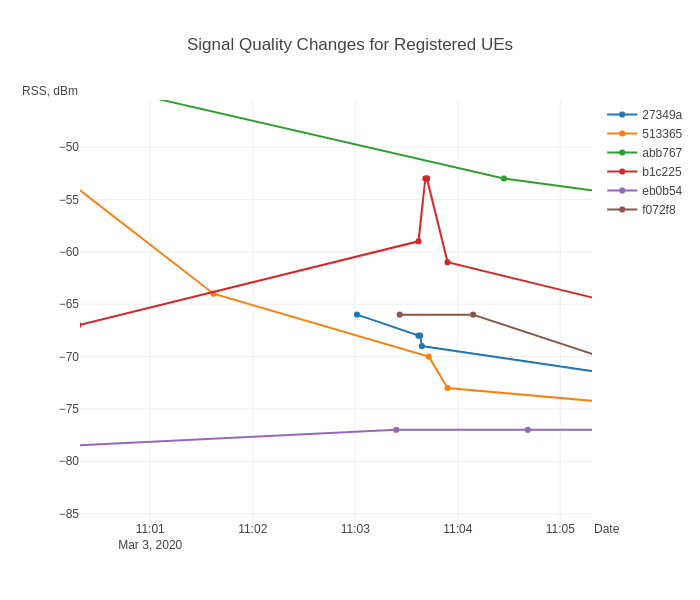
\includegraphics[width=0.7\linewidth,keepaspectratio]{images/Exp4_Suboptimal.png}
	\caption{Signal Quality changes in Sub-Optimal case}
	\label{fig:signal-quality-changes-sub-optimal}
\end{figure}

Despite the \glspl{ap} were located close to \glspl{ue}, the \acrshort{rss} level varies noticeably. However, only in this case the speed and signal quality measurement were the most stable among all cases.

\subsubsection{Uniform case}

In this case, the \glspl{ap} are located with equal distance from the \gls{command_n_center}.

\begin{figure}[H]
	\centering
	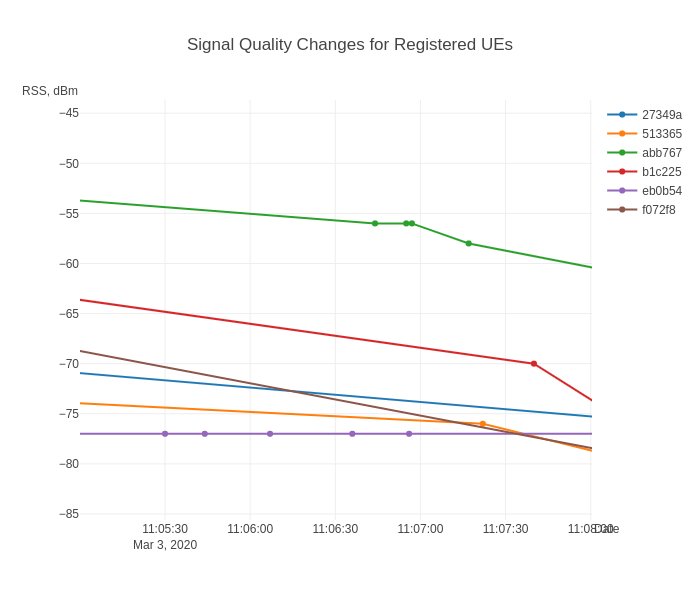
\includegraphics[width=0.7\linewidth,keepaspectratio]{images/Exp4_Uniform.png}
	\caption{Signal Quality changes in Uniform case}
	\label{fig:signal-quality-changes-uniform-optimal}
\end{figure}

Figure \ref{fig:signal-quality-changes-uniform-optimal} depict \acrshort{rss} changes in Uniform case. Link measurement is more steady and keeps on the same level for the majority of \gls{ue}, however, we encountered speed test failed.

\subsubsection{Near-optimal case}

The third case simulates the situation where the \glspl{ap} are placed
uniformly far from centers of \glspl{ue} clusters.

Figure \ref{fig:signal-quality-changes-near-optimal} demostrates that measured \acrshort{rss} lower than in Uniform case because of larger distance between \glspl{ap} and \glspl{ue} approximately on 10-15 dBm.

\begin{figure}[H]
	\centering
	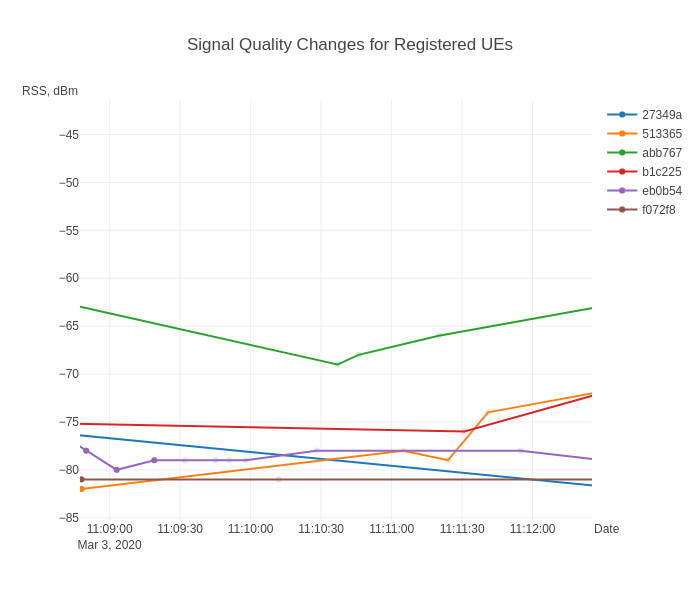
\includegraphics[width=0.7\linewidth,keepaspectratio]{images/Exp4_Near_Optimal.png}
	\caption{Signal Quality changes in Near-optimal case}
	\label{fig:signal-quality-changes-near-optimal}
\end{figure}

\subsubsection{Comparison between real coordinates in Sub-Optimal case layout and real positions
	positions}

To check the validity, we place the \glspl{ap} in a Sub-Optimal case position. Figure \ref{fig:ues-positions-for-optimization} represents the most recent positions  of \glspl{ue} as input data used for optimization tasks. The exact coordinates are presented in Table \ref{tab:exp4-sub-optimal-last-received-coordinates-ues}.

\begin{longtable}[]{@{}ll@{}}
	\caption{The last received coordinates for \glspl{ue} by \gls{gps_android}}\tabularnewline
	\toprule
	Unique ID & Coordinates\tabularnewline
	\midrule
	\endhead
	27349a2cde6592df* & 50.68206, 10.94044\tabularnewline
	51336504999bc1ca* & 50.68206, 10.94044\tabularnewline
	f072f812f48ce468* & 50.6823, 10.9406\tabularnewline
	b1c225280d0ed13f* & 50.68243, 10.94035\tabularnewline
	abb76773bdee4fa0* & 50.6823, 10.93987\tabularnewline
	eb0b54819c69cf0c* & 50.68253, 10.93984\tabularnewline
	\bottomrule
	\label{tab:exp4-sub-optimal-last-received-coordinates-ues}
\end{longtable}

\begin{figure}[H]
	\centering
	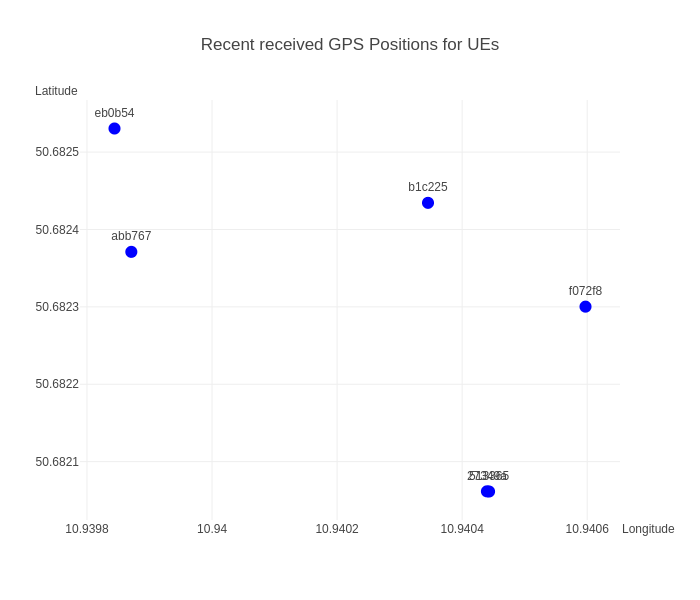
\includegraphics[width=0.5\linewidth,keepaspectratio]{images/Exp4_UEs_Location_to_optimize.png}
	\caption{The \glspl{ue} coordinates used to optimize \glspl{ap} positions}
	\label{fig:ues-positions-for-optimization}
\end{figure}

The coordinates for \textbf{27349a2cde6592df} and
\textbf{51336504999bc1ca} overlap.

The most recent received coordinates for \glspl{ue} used to schedule an optimization task with the following parameters:

\begin{itemize}
	\tightlist
	\item
	Number of clusters: 2
	\item
	Estimation method: ``clustering''
\end{itemize}

The ``simplex'' method against two clusters is not possible. Instead we use 'clustering' method which uses K-means clusterization algorithm. Figure \ref{fig:ues-positions-and-suggested-optimal-positions-for-uavs} demonstrate positions for \glspl{ue} as blue dots and suggested coordinates for two \glspl{ap} as black box.

\begin{figure}[H]
	\centering
	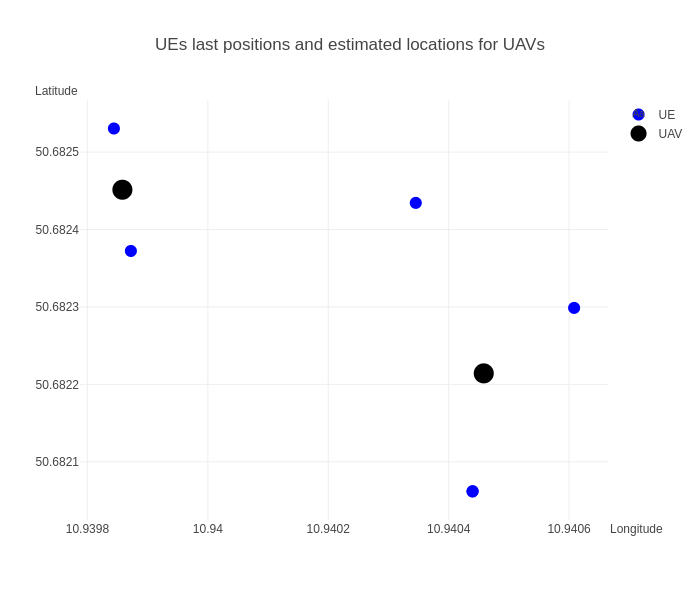
\includegraphics[width=0.5\linewidth,keepaspectratio]{images/Expt4_Estimated UAVs_locations.png}
	\caption{Result of optimization task to obtain optimal positions for \glspl{ap}}
	\label{fig:ues-positions-and-suggested-optimal-positions-for-uavs}
\end{figure}

The suggested optimal coordinates for \glspl{ap} are shown in Table \ref{tab:optimal-coordinates}.

\begin{longtable}[]{@{}lll@{}}
	\caption{Suggested optimal positions for \glspl{uav} }\tabularnewline
	\toprule
	AP & Real coordinates & Suggested coordinates\tabularnewline
	\midrule
	\endhead
	AP1 & 50.6823778, 10.94054861 & 50.68221, 10.94046\tabularnewline
	AP2 & 50.6824281, 10.940313611 & 50.68245, 10.93986\tabularnewline
	\bottomrule
	\label{tab:optimal-coordinates}
\end{longtable}

Figure \ref{fig:optimized-coordinates-on-logical-map} shows on the map real and suggested optimal coordinates for \gls{ap}. These new positions can drop out connected clients due to large distance because at this space connection became unstable, their error rate is higher.

This figure contains four types of elements:

\begin{enumerate}
	\item Green circles - represent initial coordinates for \glspl{ue}.
	
	\item Red circles - represent coordinates for \glspl{ue} received by \gls{gps_android}.
	
	\item Yellow tags - represent initial coordinates for \glspl{ap}.
	
	\item Blue tags - represent suggested optimal coordinates for \glspl{ap}.
	
\end{enumerate}

\begin{figure}[H]
	\centering
	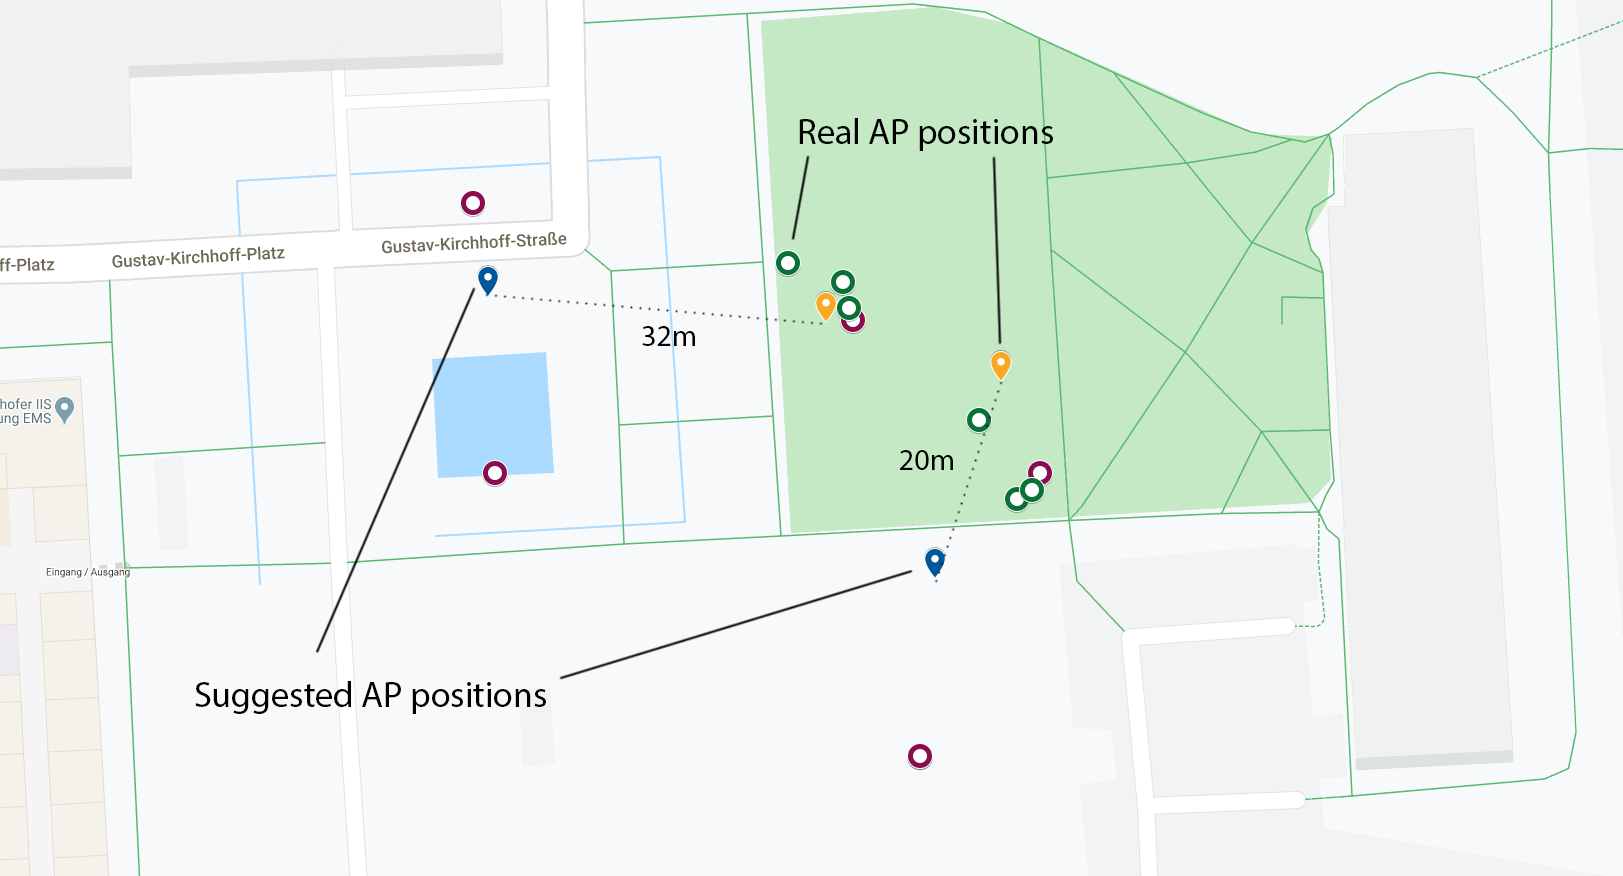
\includegraphics[width=\linewidth,keepaspectratio]{images/Expt4_Result_of_optimization_map_with_names.png}
	\caption{Original and Optimized Coordinates: A map with tags.}
	\label{fig:optimized-coordinates-on-logical-map}
\end{figure}

Distance between real and suggested positions for AP1 is 32m and 20m for AP2 accordingly. We find out two possible reasons for this difference:

\begin{enumerate}
	\item Fragmentation of used \gls{android} phones - in the experiment we used various gadgets running different \gls{os} version. They present several generations of \gls{android} evolution. The older generations can have less accurate \gls{gnss} module, therefore provide a wrong position estimate.
	\item Location provider optimization in \gls{gps_android} - \gls{gps_android} was designed  to choose between network-assisted and \acrshort{gps}-assisted location estimation. The exact option depends on what provider has better connection status. First, it tries to set up \acrshort{gps} provider, if it fails, the phone fallback to network-provided location estimation which is less accurate.
\end{enumerate}


Figure \ref{fig:optimized-coordinates-satellite-map} depict these coordinates on the map from a satellite point of view.

\begin{figure}[H]
	\centering
	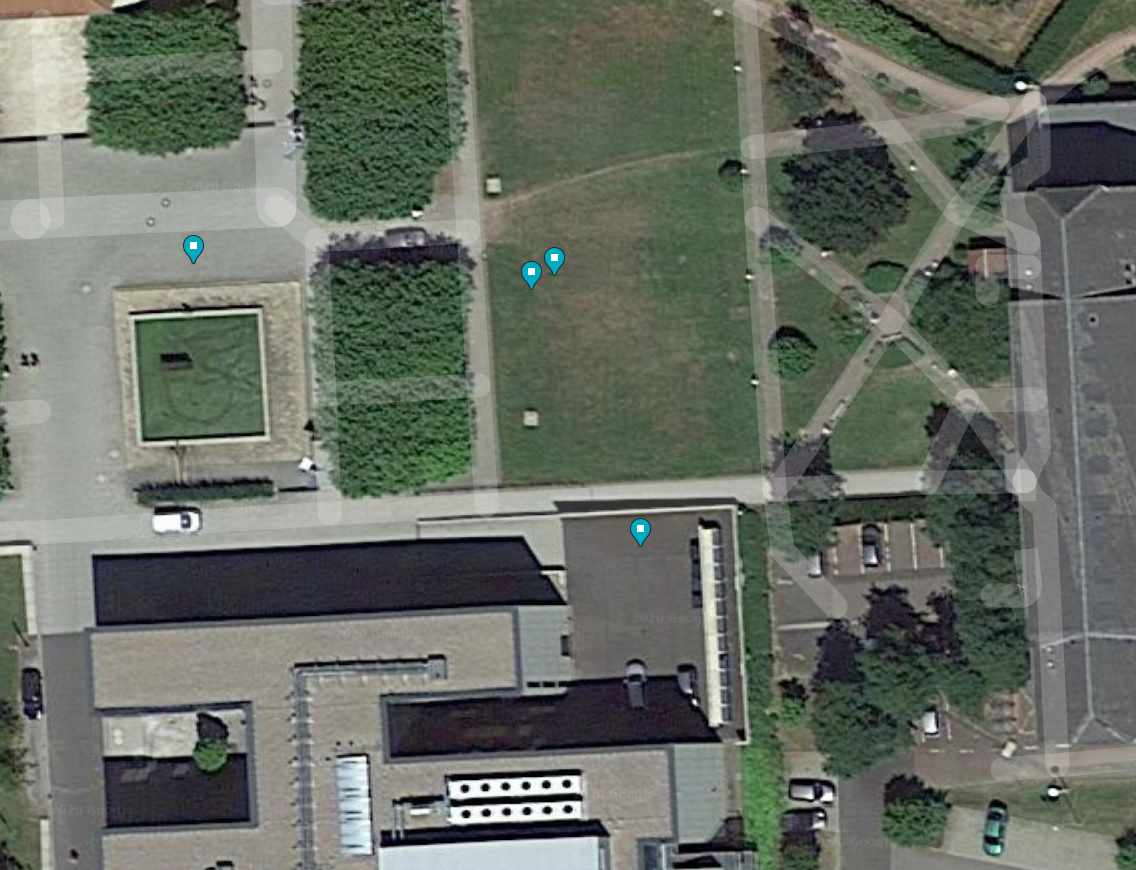
\includegraphics[width=0.5\linewidth,keepaspectratio]{images/Expt4_Result_of_optimization_sattelite.png}
	\caption{Original and Optimized Coordinates for \glspl{uav}: A map from satellites.}
	\label{fig:optimized-coordinates-satellite-map}
\end{figure}

``Clustering'' algorithm performs simple K-means cluster calculation
based on \gls{gnss} coordinates for \glspl{ue}. The result provides insights about that layout optimization algorithms relying solely on the coordinate input data can result in a biased solution.

\subsection{Outcome}

Finally, we have managed to test the framework and estimate an optimized position for \glspl{uav} which were represented by \gls{wifi} access points. The results showed that the framework match requirements, however, should be redesigned and evaluated on updated data.
